% ============================================================
%  09-release1.tex
%  Chapitre 3 : Sprints 1 et 2 -- Fondation et Gestion Client/Projet
%  Contient : Sprint 1 (Identity) + Sprint 2 (Clients & Projets)
% ============================================================
\chapter{Sprints 1 et 2~: Fondation et Gestion Client/Projet}

% ══════════════════════════════════════════════════════════
\section{Sprint 1~: Service d'Identité et Authentification}
% ══════════════════════════════════════════════════════════

\subsection{Backlog du sprint}

{\small
\setlength{\LTleft}{0pt}
\setlength{\LTright}{0pt}
\begin{longtable}{|C{0.8cm}|L{4.2cm}|>{\raggedright\arraybackslash}p{\dimexpr\textwidth-0.8cm-4.2cm-1.5cm-8\tabcolsep-5\arrayrulewidth\relax}|C{1.5cm}|}
  \caption{Backlog Kanban -- Sprint 1 (Identity Service, Port 8081)}\label{tab:backlog-s1}\\
  \hline
  \rowcolor{figblue}
  \textcolor{white}{\textbf{ID}} &
  \textcolor{white}{\textbf{User Story}} &
  \textcolor{white}{\textbf{Tâches}} &
  \textcolor{white}{\textbf{Effort}} \\
  \hline
  \endfirsthead

  \hline
  \rowcolor{figblue}
  \textcolor{white}{\textbf{ID}} &
  \textcolor{white}{\textbf{User Story}} &
  \textcolor{white}{\textbf{Tâches}} &
  \textcolor{white}{\textbf{Effort}} \\
  \hline
  \endhead

  \hline
  \multicolumn{4}{r}{\small\textit{Suite page suivante}}\\
  \endfoot

  \hline
  \endlastfoot

  1 & En tant que client, je veux créer un compte avec
    vérification e-mail pour accéder à mon espace. &
  $\rightarrow$ Endpoint \texttt{POST /register} (username, email, password, firstName, lastName, phone)\newline
  $\rightarrow$ Hash BCrypt (force 10)\newline
  $\rightarrow$ Rôle automatiquement assigné à \texttt{CLIENT}\newline
  $\rightarrow$ Génération OTP 6 chiffres (TTL 10 min)\newline
  $\rightarrow$ Envoi OTP par e-mail (SMTP)\newline
  $\rightarrow$ Endpoints \texttt{POST /verify-otp} et \texttt{POST /resend-otp}\newline
  $\rightarrow$ Interface React (formulaire + page OTP)\newline
  $\rightarrow$ Tests unitaires et intégration & Élevé \\
  \hline
  2 & En tant qu'admin, je veux créer et gérer les comptes
    installateurs de l'entreprise. &
  $\rightarrow$ Endpoint \texttt{POST /api/auth/installers} (firstName, lastName, email, phone, password)\newline
  $\rightarrow$ Endpoints \texttt{GET}, \texttt{PUT}, \texttt{DELETE /api/auth/installers/\{uuid\}}\newline
  $\rightarrow$ Compte créé directement vérifié (\texttt{isEmailVerified=true})\newline
  $\rightarrow$ Interface admin de gestion des installateurs\newline
  $\rightarrow$ Vérification du rôle \texttt{ADMIN} obligatoire & Élevé \\
  \hline
  3 & En tant qu'utilisateur (client ou installateur), je veux me connecter
    et obtenir un token JWT pour accéder aux services. &
  $\rightarrow$ Endpoint \texttt{POST /login}\newline
  $\rightarrow$ Génération Access Token (HS256, 1h) avec claims \texttt{role}, \texttt{email}\newline
  $\rightarrow$ Génération Refresh Token (UUID, 7j)\newline
  $\rightarrow$ Endpoint \texttt{POST /refresh} (rotation)\newline
  $\rightarrow$ Réponse \texttt{AuthResponse} enrichie (tokens + \texttt{UserDto})\newline
  $\rightarrow$ Interface login React + redirection selon le rôle\newline
  $\rightarrow$ Tests avec Postman & Élevé \\
  \hline
  4 & En tant qu'utilisateur connecté, je veux consulter et
    modifier mon profil. &
  $\rightarrow$ Endpoints \texttt{GET /me} et \texttt{PUT /me}\newline
  $\rightarrow$ Endpoint dédié \texttt{PUT /me/password} (ancien + nouveau mot de passe)\newline
  $\rightarrow$ Interface profil React\newline
  $\rightarrow$ Tests fonctionnels & Moyen \\
  \hline
  5 & En tant que système, le Gateway doit valider les JWT
    et propager l'identité aux services. &
  $\rightarrow$ Filtre JWT dans Spring Cloud Gateway\newline
  $\rightarrow$ Propagation \texttt{X-User-Id}, \texttt{X-User-Role}, \texttt{X-User-Email}\newline
  $\rightarrow$ Liste de routes publiques exemptées (register, login, OTP, etc.)\newline
  $\rightarrow$ Rejet automatique des tokens expirés (HTTP 401)\newline
  $\rightarrow$ Tests de sécurité (token valide/invalide) & Élevé \\
  \hline
\end{longtable}
}

\subsection{Analyse du sprint 1}

Pour mieux comprendre ce premier sprint, nous allons présenter le diagramme
de cas d'utilisation du sprint~1, décrire les différents cas d'utilisation,
et détailler les fonctionnalités mentionnées dans ce sprint.

\subsubsection{Diagramme de cas d'utilisation global relatif au sprint 1}

Ce diagramme de cas d'utilisation illustre les différentes fonctionnalités
prises en charge lors du sprint~1, accessibles aux deux acteurs principaux~:
l'\textbf{Admin}, qui crée et gère les comptes installateurs en interne, et
le \textbf{Client}, qui s'auto-inscrit via le formulaire public et gère son
propre profil. Les installateurs ne s'inscrivent pas eux-mêmes~; leurs comptes
sont provisionnés par l'administrateur.

\begin{figure}[H]
  \centering
  \IfFileExists{101.png}{%
    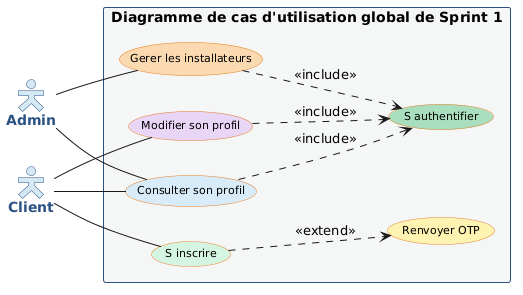
\includegraphics[width=0.88\textwidth]{101.png}%
  }{%
    \fbox{\parbox[c][8cm][c]{0.92\textwidth}{\centering Diagramme de cas d'utilisation global de Sprint 1}}%
  }
  \caption{Diagramme de cas d'utilisation global de Sprint~1}
  \label{fig:uc-s1}
\end{figure}

\subsubsection{Vue détaillée des cas d'utilisation développés durant le sprint 1}

Ensuite, nous présentons les diagrammes de cas d'utilisation détaillés
correspondant aux fonctionnalités principales. Ces diagrammes permettent
de mieux illustrer les interactions entre les acteurs et le système.

% ──────────────────────────────────────────────
\paragraph{Raffinement de cas d'utilisation «~Gérer les installateurs~»}

\begin{figure}[H]
  \centering
  \IfFileExists{102.png}{%
    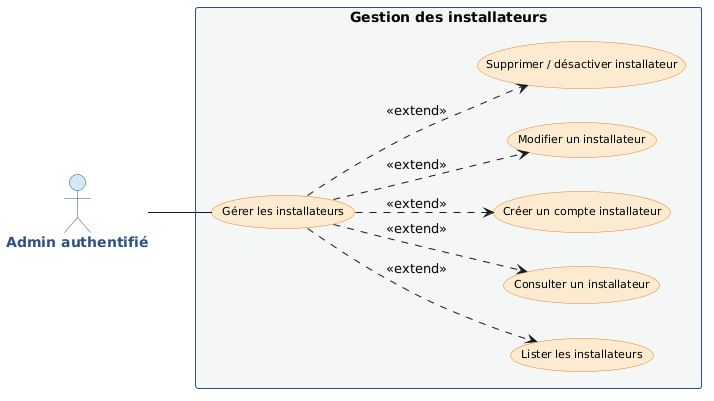
\includegraphics[width=0.85\textwidth]{102.png}%
  }{%
    \fbox{\parbox[c][6cm][c]{0.85\textwidth}{\centering Diagramme de cas d'utilisation -- Gérer les installateurs}}%
  }
  \caption{Diagramme de cas d'utilisation pour «~Gérer les installateurs~»}
  \label{fig:uc-installateurs}
\end{figure}

\subparagraph{Description textuelle du cas d'utilisation «~Créer un compte installateur~»}

\begin{table}[H]
  \caption{Description textuelle du cas d'utilisation «~Créer un compte installateur~»}
  \label{tab:cu-creer-installateur}
  \centering
  \begin{tabularx}{\textwidth}{|L{3.8cm}|X|}
    \hline
    \rowcolor{figblue!10}
    \textbf{Cas d'utilisation} & Créer un compte installateur. \\
    \hline
    \textbf{Acteur initiateur} & Administrateur \\
    \hline
    \textbf{But du cas} & Permettre à l'administrateur d'ajouter un nouveau compte installateur au système en saisissant les informations requises. \\
    \hline
    \textbf{Précondition} & L'administrateur doit être authentifié avec succès, l'e-mail de l'installateur n'existe pas dans la base. \\
    \hline
    \textbf{Description du scénario} &
    \textbf{Scénario principal :}\newline
    1. L'administrateur se connecte au système via l'interface d'authentification.\newline
    2. Il accède à la section «~Gestion des installateurs~».\newline
    3. Il clique sur le bouton «~Créer un compte installateur~».\newline
    4. Un formulaire d'ajout s'affiche.\newline
    5. L'administrateur saisit les informations nécessaires (prénom, nom, e-mail, téléphone, mot de passe).\newline
    6. Il valide le formulaire.\newline
    7. Le système hache le mot de passe (BCrypt, force~10) et enregistre le compte avec \texttt{isEmailVerified=true}, rôle \texttt{INSTALLER}.\newline
    8. Le système affiche un message de confirmation et met à jour la liste des installateurs.\\
    \hline
    \textbf{Scénarios alternatifs} &
    \textit{Scénario alternatif 1 -- Installateur déjà existant :}\newline
    \hspace*{6pt}7.1.~L'administrateur saisit un e-mail déjà enregistré.\newline
    \hspace*{6pt}7.2.~Le système affiche un message d'erreur~: «~Installateur déjà existant~».\newline[2pt]
    \textit{Scénario alternatif 2 -- Rôle insuffisant :}\newline
    \hspace*{6pt}1.1.~Un utilisateur non administrateur tente d'accéder à la route.\newline
    \hspace*{6pt}1.2.~Le Gateway renvoie HTTP~403 et refuse l'accès.\\
    \hline
  \end{tabularx}
\end{table}

\subparagraph{Description textuelle du cas d'utilisation «~Modifier un installateur~»}

\begin{table}[H]
  \caption{Description textuelle du cas d'utilisation «~Modifier un installateur~»}
  \label{tab:cu-modifier-installateur}
  \centering
  \begin{tabularx}{\textwidth}{|L{3.8cm}|X|}
    \hline
    \rowcolor{figblue!10}
    \textbf{Cas d'utilisation} & Modifier un installateur. \\
    \hline
    \textbf{Acteur initiateur} & Administrateur \\
    \hline
    \textbf{But du cas} & Permettre à l'administrateur de modifier les informations d'un compte installateur déjà existant (nom, prénom, téléphone, e-mail, statut actif). \\
    \hline
    \textbf{Précondition} & L'administrateur est authentifié et l'installateur ciblé existe dans la base. \\
    \hline
    \textbf{Description du scénario} &
    \textbf{Scénario principal :}\newline
    1. L'administrateur se connecte au système.\newline
    2. Il accède à la section «~Gestion des installateurs~».\newline
    3. Le système affiche la liste des installateurs.\newline
    4. L'administrateur sélectionne un installateur à modifier.\newline
    5. Il saisit les modifications souhaitées dans le formulaire prérempli.\newline
    6. Le système valide les nouvelles données.\newline
    7. Le système enregistre les modifications et affiche un message de confirmation.\newline
    8. La liste des installateurs est mise à jour.\\
    \hline
    \textbf{Scénarios alternatifs} &
    \textit{Scénario alternatif 1 -- Installateur introuvable :}\newline
    \hspace*{6pt}4.1.~L'identifiant ne correspond à aucun installateur.\newline
    \hspace*{6pt}4.2.~Le système renvoie HTTP~404 : «~Installateur introuvable~».\newline[2pt]
    \textit{Scénario alternatif 2 -- E-mail déjà utilisé :}\newline
    \hspace*{6pt}6.1.~Le nouvel e-mail est déjà attribué à un autre compte.\newline
    \hspace*{6pt}6.2.~Le système renvoie HTTP~409 et affiche un message d'erreur.\\
    \hline
  \end{tabularx}
\end{table}

\subparagraph{Description textuelle du cas d'utilisation «~Supprimer / désactiver un installateur~»}

\begin{table}[H]
  \caption{Description textuelle du cas d'utilisation «~Supprimer / désactiver un installateur~»}
  \label{tab:cu-supprimer-installateur}
  \centering
  \begin{tabularx}{\textwidth}{|L{3.8cm}|X|}
    \hline
    \rowcolor{figblue!10}
    \textbf{Cas d'utilisation} & Supprimer / désactiver un installateur. \\
    \hline
    \textbf{Acteur initiateur} & Administrateur \\
    \hline
    \textbf{But du cas} & Permettre à l'administrateur de retirer un installateur de la plateforme par une suppression logique (\texttt{isActive=false}), préservant ainsi l'historique des projets et clients associés. \\
    \hline
    \textbf{Précondition} & L'administrateur est authentifié et l'installateur ciblé existe. \\
    \hline
    \textbf{Description du scénario} &
    \textbf{Scénario principal :}\newline
    1. L'administrateur accède à la section «~Gestion des installateurs~».\newline
    2. Le système affiche la liste des installateurs.\newline
    3. L'administrateur sélectionne un installateur à désactiver.\newline
    4. Il clique sur le bouton «~Désactiver~».\newline
    5. Le système demande une confirmation.\newline
    6. L'administrateur confirme l'action.\newline
    7. Le système met à jour le statut (\texttt{isActive=false}) et révoque tous les Refresh Tokens de l'installateur.\newline
    8. Un message de confirmation s'affiche.\\
    \hline
    \textbf{Scénarios alternatifs} &
    \textit{Scénario alternatif 1 -- Annulation :}\newline
    \hspace*{6pt}5.1.~L'administrateur annule la confirmation.\newline
    \hspace*{6pt}5.2.~Aucune modification n'est appliquée.\newline[2pt]
    \textit{Scénario alternatif 2 -- Installateur avec projets actifs :}\newline
    \hspace*{6pt}6.1.~Le système alerte sur la présence de projets en cours.\newline
    \hspace*{6pt}6.2.~L'administrateur doit confirmer ou réaffecter les projets avant désactivation.\\
    \hline
  \end{tabularx}
\end{table}

\subparagraph{Description textuelle du cas d'utilisation «~Lister les installateurs~»}

\begin{table}[H]
  \caption{Description textuelle du cas d'utilisation «~Lister les installateurs~»}
  \label{tab:cu-lister-installateurs}
  \centering
  \begin{tabularx}{\textwidth}{|L{3.8cm}|X|}
    \hline
    \rowcolor{figblue!10}
    \textbf{Cas d'utilisation} & Lister les installateurs. \\
    \hline
    \textbf{Acteur initiateur} & Administrateur \\
    \hline
    \textbf{But du cas} & Permettre à l'administrateur de visualiser l'ensemble des comptes installateurs enregistrés, avec leurs informations principales (nom, e-mail, statut, date de création). \\
    \hline
    \textbf{Précondition} & L'administrateur doit être authentifié avec succès. \\
    \hline
    \textbf{Description du scénario} &
    \textbf{Scénario principal :}\newline
    1. L'administrateur se connecte au système.\newline
    2. Il accède à la section «~Gestion des installateurs~».\newline
    3. Le système envoie une requête \texttt{GET /api/auth/installers}.\newline
    4. Le système récupère tous les utilisateurs de rôle \texttt{INSTALLER}.\newline
    5. La liste est affichée sous forme de tableau paginé avec filtres (statut, recherche par nom).\newline
    6. L'administrateur peut trier, filtrer ou cliquer sur un installateur pour le consulter.\\
    \hline
    \textbf{Scénarios alternatifs} &
    \textit{Scénario alternatif 1 -- Aucun installateur :}\newline
    \hspace*{6pt}5.1.~La base ne contient aucun installateur.\newline
    \hspace*{6pt}5.2.~Le système affiche : «~Aucun installateur enregistré~».\newline[2pt]
    \textit{Scénario alternatif 2 -- Erreur serveur :}\newline
    \hspace*{6pt}3.1.~Le service d'identité est indisponible.\newline
    \hspace*{6pt}3.2.~Le système affiche un message d'erreur et propose de réessayer.\\
    \hline
  \end{tabularx}
\end{table}

% ──────────────────────────────────────────────
\paragraph{Raffinement de cas d'utilisation «~S'inscrire~»}

\begin{figure}[H]
  \centering
  \IfFileExists{103.png}{%
    \includegraphics[width=0.85\textwidth]{103.png}%
  }{%
    \fbox{\parbox[c][6cm][c]{0.85\textwidth}{\centering Diagramme de cas d'utilisation -- S'inscrire}}%
  }
  \caption{Diagramme de cas d'utilisation pour «~S'inscrire~»}
  \label{fig:uc-sinscrire}
\end{figure}

\subparagraph{Description textuelle du cas d'utilisation «~S'inscrire~»}

\begin{table}[H]
  \caption{Description textuelle du cas d'utilisation «~S'inscrire~»}
  \label{tab:cu-sinscrire}
  \centering
  \begin{tabularx}{\textwidth}{|L{3.8cm}|X|}
    \hline
    \rowcolor{figblue!10}
    \textbf{Cas d'utilisation} & S'inscrire sur la plateforme SolarEase. \\
    \hline
    \textbf{Acteur initiateur} & Visiteur (futur client) \\
    \hline
    \textbf{But du cas} & Permettre à un visiteur de créer un compte client en vérifiant son adresse e-mail par un code OTP, afin d'accéder à son espace personnel. \\
    \hline
    \textbf{Précondition} & L'adresse e-mail n'existe pas déjà dans la base. \\
    \hline
    \textbf{Description du scénario} &
    \textbf{Scénario principal :}\newline
    1. Le visiteur accède au formulaire d'inscription public.\newline
    2. Il saisit ses informations (nom, prénom, e-mail, téléphone, mot de passe).\newline
    3. Le système valide les champs et hache le mot de passe (BCrypt, force~10).\newline
    4. Le compte est créé avec \texttt{isEmailVerified=false} et rôle \texttt{CLIENT}.\newline
    5. Le système génère un code OTP à 6~chiffres (TTL 10~min) et l'envoie par e-mail.\newline
    6. Le visiteur est redirigé vers la page de vérification OTP.\newline
    7. Il saisit le code reçu.\newline
    8. Le système valide l'OTP et active le compte (\texttt{isEmailVerified=true}).\newline
    9. Le visiteur peut alors se connecter.\\
    \hline
    \textbf{Scénarios alternatifs} &
    \textit{Scénario alternatif 1 -- E-mail déjà utilisé :}\newline
    \hspace*{6pt}3.1.~Le système détecte un e-mail existant et renvoie HTTP~409.\newline[2pt]
    \textit{Scénario alternatif 2 -- OTP expiré :}\newline
    \hspace*{6pt}7.1.~Le code saisi est expiré ($>$10~min).\newline
    \hspace*{6pt}7.2.~Le système propose le renvoi d'un nouveau code (\texttt{POST /resend-otp}).\\
    \hline
  \end{tabularx}
\end{table}

\subparagraph{Description textuelle du cas d'utilisation «~Vérifier le code OTP~»}

\begin{table}[H]
  \caption{Description textuelle du cas d'utilisation «~Vérifier le code OTP~»}
  \label{tab:cu-verifier-otp}
  \centering
  \begin{tabularx}{\textwidth}{|L{3.8cm}|X|}
    \hline
    \rowcolor{figblue!10}
    \textbf{Cas d'utilisation} & Vérifier le code OTP. \\
    \hline
    \textbf{Acteur initiateur} & Visiteur inscrit (compte non encore activé) \\
    \hline
    \textbf{But du cas} & Permettre au visiteur d'activer son compte en confirmant la réception du code OTP envoyé à son adresse e-mail. \\
    \hline
    \textbf{Précondition} & Le compte existe avec \texttt{isEmailVerified=false} et un OTP valide est présent en base (non utilisé et non expiré). \\
    \hline
    \textbf{Description du scénario} &
    \textbf{Scénario principal :}\newline
    1. Le visiteur est redirigé sur la page de vérification.\newline
    2. Il consulte sa boîte e-mail et récupère le code à 6~chiffres.\newline
    3. Il saisit le code dans le formulaire.\newline
    4. Le système recherche l'OTP en base (par e-mail + code).\newline
    5. Vérification : token non utilisé et non expiré ($<$10~min).\newline
    6. Le système marque l'OTP comme utilisé (\texttt{used=true}).\newline
    7. Le compte est activé (\texttt{isEmailVerified=true}).\newline
    8. Un message de confirmation est affiché et l'utilisateur est redirigé vers la page de connexion.\\
    \hline
    \textbf{Scénarios alternatifs} &
    \textit{Scénario alternatif 1 -- Code incorrect :}\newline
    \hspace*{6pt}4.1.~Aucun OTP ne correspond au code saisi.\newline
    \hspace*{6pt}4.2.~Le système renvoie HTTP~400 : «~Code OTP incorrect~».\newline[2pt]
    \textit{Scénario alternatif 2 -- OTP expiré :}\newline
    \hspace*{6pt}5.1.~L'OTP est en base mais expiré.\newline
    \hspace*{6pt}5.2.~Le système propose de demander un nouveau code.\newline[2pt]
    \textit{Scénario alternatif 3 -- OTP déjà utilisé :}\newline
    \hspace*{6pt}5.3.~Le champ \texttt{used} est déjà à \texttt{true}.\newline
    \hspace*{6pt}5.4.~Le système rejette la requête.\\
    \hline
  \end{tabularx}
\end{table}

\subparagraph{Description textuelle du cas d'utilisation «~Renvoyer un OTP~»}

\begin{table}[H]
  \caption{Description textuelle du cas d'utilisation «~Renvoyer un OTP~»}
  \label{tab:cu-renvoyer-otp}
  \centering
  \begin{tabularx}{\textwidth}{|L{3.8cm}|X|}
    \hline
    \rowcolor{figblue!10}
    \textbf{Cas d'utilisation} & Renvoyer un code OTP. \\
    \hline
    \textbf{Acteur initiateur} & Visiteur inscrit (compte non activé) \\
    \hline
    \textbf{But du cas} & Permettre au visiteur de demander un nouveau code OTP s'il n'a pas reçu le précédent ou si celui-ci a expiré. \\
    \hline
    \textbf{Précondition} & Le compte existe avec \texttt{isEmailVerified=false}. \\
    \hline
    \textbf{Description du scénario} &
    \textbf{Scénario principal :}\newline
    1. Le visiteur clique sur le lien «~Renvoyer le code~» dans la page de vérification.\newline
    2. Le système vérifie le délai anti-flood (1 demande / 60~secondes).\newline
    3. L'ancien OTP est invalidé (\texttt{used=true}).\newline
    4. Le système génère un nouveau code à 6~chiffres avec un nouveau TTL de 10~minutes.\newline
    5. Le code est enregistré en base et envoyé par e-mail.\newline
    6. Un message de confirmation s'affiche : «~Code renvoyé~».\\
    \hline
    \textbf{Scénarios alternatifs} &
    \textit{Scénario alternatif 1 -- Anti-flood actif :}\newline
    \hspace*{6pt}2.1.~Une demande a déjà été faite il y a moins de 60~secondes.\newline
    \hspace*{6pt}2.2.~Le système renvoie HTTP~429 : «~Veuillez patienter avant de redemander un code~».\newline[2pt]
    \textit{Scénario alternatif 2 -- Compte déjà activé :}\newline
    \hspace*{6pt}1.1.~Le compte est déjà vérifié.\newline
    \hspace*{6pt}1.2.~Le système redirige vers la page de connexion.\\
    \hline
  \end{tabularx}
\end{table}

% ──────────────────────────────────────────────
\paragraph{Raffinement de cas d'utilisation «~Modifier son profil~»}

\begin{figure}[H]
  \centering
  \IfFileExists{104.png}{%
    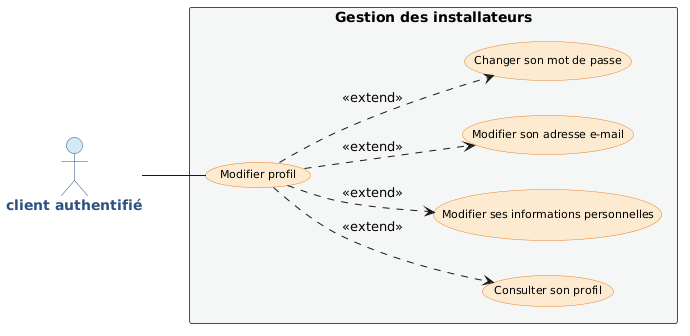
\includegraphics[width=0.85\textwidth]{104.png}%
  }{%
    \fbox{\parbox[c][6cm][c]{0.85\textwidth}{\centering Diagramme de cas d'utilisation -- Modifier son profil}}%
  }
  \caption{Diagramme de cas d'utilisation pour «~Modifier son profil~»}
  \label{fig:uc-profil}
\end{figure}

\subparagraph{Description textuelle du cas d'utilisation «~Changer son mot de passe~»}

\begin{table}[H]
  \caption{Description textuelle du cas d'utilisation «~Changer son mot de passe~»}
  \label{tab:cu-changer-mdp}
  \centering
  \begin{tabularx}{\textwidth}{|L{3.8cm}|X|}
    \hline
    \rowcolor{figblue!10}
    \textbf{Cas d'utilisation} & Changer son mot de passe. \\
    \hline
    \textbf{Acteur initiateur} & Client (ou tout utilisateur authentifié) \\
    \hline
    \textbf{But du cas} & Permettre à un utilisateur authentifié de modifier son mot de passe afin de renforcer la sécurité de son compte. \\
    \hline
    \textbf{Précondition} & L'utilisateur est authentifié et connaît son ancien mot de passe. \\
    \hline
    \textbf{Description du scénario} &
    \textbf{Scénario principal :}\newline
    1. L'utilisateur s'authentifie dans le système.\newline
    2. Il accède à la section «~Mon profil~».\newline
    3. Il clique sur «~Changer mot de passe~».\newline
    4. Il saisit son ancien mot de passe puis le nouveau (deux fois).\newline
    5. Le système vérifie l'ancien mot de passe (comparaison BCrypt).\newline
    6. Le système valide la force du nouveau mot de passe ($\geq$~8 caractères).\newline
    7. Le nouveau mot de passe est haché et enregistré.\newline
    8. Tous les Refresh Tokens existants sont révoqués.\newline
    9. Le système envoie une notification e-mail d'alerte sécurité.\newline
    10. Un message de confirmation s'affiche.\\
    \hline
    \textbf{Scénarios alternatifs} &
    \textit{Scénario alternatif 1 -- Ancien mot de passe incorrect :}\newline
    \hspace*{6pt}5.1.~Le système renvoie HTTP~401.\newline
    \hspace*{6pt}5.2.~Le formulaire affiche~: «~Ancien mot de passe incorrect~».\newline[2pt]
    \textit{Scénario alternatif 2 -- Nouveau mot de passe trop faible :}\newline
    \hspace*{6pt}6.1.~Le système renvoie une erreur de validation.\newline
    \hspace*{6pt}6.2.~Le formulaire indique les exigences (longueur, complexité).\\
    \hline
  \end{tabularx}
\end{table}

\subparagraph{Description textuelle du cas d'utilisation «~Modifier son adresse e-mail~»}

\begin{table}[H]
  \caption{Description textuelle du cas d'utilisation «~Modifier son adresse e-mail~»}
  \label{tab:cu-modifier-email}
  \centering
  \begin{tabularx}{\textwidth}{|L{3.8cm}|X|}
    \hline
    \rowcolor{figblue!10}
    \textbf{Cas d'utilisation} & Modifier son adresse e-mail. \\
    \hline
    \textbf{Acteur initiateur} & Utilisateur authentifié (Client, Installateur ou Admin) \\
    \hline
    \textbf{But du cas} & Permettre à l'utilisateur de changer l'adresse e-mail associée à son compte avec re-vérification obligatoire par OTP. \\
    \hline
    \textbf{Précondition} & L'utilisateur est authentifié et la nouvelle adresse n'est pas déjà utilisée par un autre compte. \\
    \hline
    \textbf{Description du scénario} &
    \textbf{Scénario principal :}\newline
    1. L'utilisateur accède à la section «~Mon profil~».\newline
    2. Il clique sur «~Modifier mon e-mail~».\newline
    3. Il saisit la nouvelle adresse e-mail.\newline
    4. Le système valide le format et l'unicité de l'adresse.\newline
    5. Le système génère un OTP de confirmation et l'envoie à la nouvelle adresse.\newline
    6. L'utilisateur récupère le code et le saisit.\newline
    7. Le système valide l'OTP et applique la nouvelle adresse (\texttt{user.email = nouveau}).\newline
    8. Tous les Refresh Tokens existants sont révoqués.\newline
    9. Un message de confirmation est affiché.\\
    \hline
    \textbf{Scénarios alternatifs} &
    \textit{Scénario alternatif 1 -- E-mail déjà utilisé :}\newline
    \hspace*{6pt}4.1.~La nouvelle adresse appartient à un autre compte.\newline
    \hspace*{6pt}4.2.~Le système renvoie HTTP~409 : «~Cette adresse e-mail est déjà utilisée~».\newline[2pt]
    \textit{Scénario alternatif 2 -- OTP non saisi à temps :}\newline
    \hspace*{6pt}6.1.~L'utilisateur n'a pas validé l'OTP dans les 10~minutes.\newline
    \hspace*{6pt}6.2.~La nouvelle adresse n'est pas appliquée, l'ancienne reste active.\\
    \hline
  \end{tabularx}
\end{table}

\subparagraph{Description textuelle du cas d'utilisation «~Modifier ses informations personnelles~»}

\begin{table}[H]
  \caption{Description textuelle du cas d'utilisation «~Modifier ses informations personnelles~»}
  \label{tab:cu-modifier-infos}
  \centering
  \begin{tabularx}{\textwidth}{|L{3.8cm}|X|}
    \hline
    \rowcolor{figblue!10}
    \textbf{Cas d'utilisation} & Modifier ses informations personnelles. \\
    \hline
    \textbf{Acteur initiateur} & Utilisateur authentifié \\
    \hline
    \textbf{But du cas} & Permettre à l'utilisateur de mettre à jour ses informations personnelles (prénom, nom, téléphone, adresse postale) sans validation supplémentaire par OTP. \\
    \hline
    \textbf{Précondition} & L'utilisateur est authentifié avec succès. \\
    \hline
    \textbf{Description du scénario} &
    \textbf{Scénario principal :}\newline
    1. L'utilisateur accède à la section «~Mon profil~».\newline
    2. Le système affiche le formulaire prérempli avec ses informations actuelles.\newline
    3. L'utilisateur modifie les champs souhaités (prénom, nom, téléphone, adresse).\newline
    4. Il valide le formulaire.\newline
    5. Le système valide les données (Jakarta Validation).\newline
    6. Les nouvelles informations sont enregistrées en base.\newline
    7. Un message de confirmation est affiché.\\
    \hline
    \textbf{Scénarios alternatifs} &
    \textit{Scénario alternatif 1 -- Données invalides :}\newline
    \hspace*{6pt}5.1.~Le numéro de téléphone est mal formé ou un champ obligatoire est vide.\newline
    \hspace*{6pt}5.2.~Le système renvoie HTTP~400 avec le détail des erreurs.\newline
    \hspace*{6pt}5.3.~L'utilisateur corrige et revient à l'étape~4.\\
    \hline
  \end{tabularx}
\end{table}

\subparagraph{Description textuelle du cas d'utilisation «~Consulter son profil~»}

\begin{table}[H]
  \caption{Description textuelle du cas d'utilisation «~Consulter son profil~»}
  \label{tab:cu-consulter-profil}
  \centering
  \begin{tabularx}{\textwidth}{|L{3.8cm}|X|}
    \hline
    \rowcolor{figblue!10}
    \textbf{Cas d'utilisation} & Consulter son profil. \\
    \hline
    \textbf{Acteur initiateur} & Utilisateur authentifié \\
    \hline
    \textbf{But du cas} & Permettre à l'utilisateur de visualiser l'ensemble des informations de son compte (sans exposer les données sensibles). \\
    \hline
    \textbf{Précondition} & L'utilisateur est authentifié avec un JWT valide. \\
    \hline
    \textbf{Description du scénario} &
    \textbf{Scénario principal :}\newline
    1. L'utilisateur accède à la section «~Mon profil~».\newline
    2. Le frontend envoie une requête \texttt{GET /api/auth/me}.\newline
    3. Le Gateway valide le JWT et propage l'identifiant.\newline
    4. Le système récupère l'utilisateur en base.\newline
    5. Le système retourne un \texttt{UserDto} (id, e-mail, prénom, nom, téléphone, rôle, date de création).\newline
    6. Le frontend affiche les informations dans la page «~Mon profil~».\\
    \hline
    \textbf{Scénarios alternatifs} &
    \textit{Scénario alternatif 1 -- Session expirée :}\newline
    \hspace*{6pt}3.1.~Le JWT est expiré ou invalide.\newline
    \hspace*{6pt}3.2.~Le Gateway renvoie HTTP~401.\newline
    \hspace*{6pt}3.3.~Le frontend tente un \texttt{refresh} automatique, sinon redirige vers la page de connexion.\\
    \hline
  \end{tabularx}
\end{table}

\subsection{Conception du sprint 1}

L'analyse conceptuelle de ce premier sprint comprendra la description des
diagrammes de séquence liés aux fonctionnalités majeures du sprint~1. Elle
se conclura par l'élaboration du diagramme de classes, synthétisant
l'ensemble des éléments étudiés.

\subsubsection{Diagrammes de séquence}

Dans cette phase, nous présentons les diagrammes de séquence correspondant
aux principales fonctionnalités développées lors du sprint~1. Ces diagrammes
illustrent les interactions entre les différents composants du système pour
chaque fonctionnalité ciblée.

% ──────────────────────────────────────────────
\paragraph{Diagramme de séquence «~S'authentifier~»}

La figure ci-après présente le scénario de connexion d'un utilisateur
(Admin, Installateur ou Client) avec génération d'un JWT par le service
d'identité.

\begin{figure}[H]
  \centering
  \IfFileExists{seq-sauthentifier.png}{%
    \includegraphics[width=0.95\textwidth,height=0.55\textheight,keepaspectratio]{seq-sauthentifier.png}%
  }{%
    \fbox{\parbox[c][7cm][c]{0.92\textwidth}{\centering Diagramme de séquence «~S'authentifier~»}}%
  }
  \caption{Diagramme de séquence «~S'authentifier~»}
  \label{fig:seq-sauthentifier}
\end{figure}

% ──────────────────────────────────────────────
\paragraph{Diagramme de séquence «~Créer un compte installateur~»}

La figure ci-après présente le cas d'utilisation de la création d'un
compte installateur par l'administrateur.

\begin{figure}[H]
  \centering
  \IfFileExists{seq-creer-installateur.png}{%
    \includegraphics[width=0.95\textwidth,height=0.55\textheight,keepaspectratio]{seq-creer-installateur.png}%
  }{%
    \fbox{\parbox[c][7cm][c]{0.92\textwidth}{\centering Diagramme de séquence «~Créer un compte installateur~»}}%
  }
  \caption{Diagramme de séquence «~Créer un compte installateur~»}
  \label{fig:seq-creer-installateur}
\end{figure}

% ──────────────────────────────────────────────
\paragraph{Diagramme de séquence «~S'inscrire~»}

La figure ci-après présente le cas d'utilisation de l'inscription d'un
client avec génération et vérification du code OTP.

\begin{figure}[H]
  \centering
  \IfFileExists{seq-sinscrire.png}{%
    \includegraphics[width=0.95\textwidth,height=0.7\textheight,keepaspectratio]{seq-sinscrire.png}%
  }{%
    \fbox{\parbox[c][8cm][c]{0.92\textwidth}{\centering Diagramme de séquence «~S'inscrire~»}}%
  }
  \caption{Diagramme de séquence «~S'inscrire~»}
  \label{fig:seq-sinscrire}
\end{figure}

% ──────────────────────────────────────────────
\paragraph{Diagramme de séquence «~Changer son mot de passe~»}

La figure ci-après présente le cas d'utilisation de la modification du
mot de passe par un utilisateur authentifié.

\begin{figure}[H]
  \centering
  \IfFileExists{seq-changer-mdp.png}{%
    \includegraphics[width=0.95\textwidth,height=0.6\textheight,keepaspectratio]{seq-changer-mdp.png}%
  }{%
    \fbox{\parbox[c][7cm][c]{0.92\textwidth}{\centering Diagramme de séquence «~Changer son mot de passe~»}}%
  }
  \caption{Diagramme de séquence «~Changer son mot de passe~»}
  \label{fig:seq-changer-mdp}
\end{figure}

\subsubsection{Diagramme de classes du sprint 1}

Ce diagramme de classes global illustre l'architecture du projet, avec les
classes liées au sprint~1.

Il permet d'identifier clairement les entités utilisées lors de ce premier
sprint.

\begin{figure}[H]
  \centering
  \includegraphics[width=0.85\textwidth]{class-sprint1.png}
  \caption{Diagramme de classes global du sprint~1}
  \label{fig:class-s1}
\end{figure}

\subsection{Réalisation du sprint 1}

Cette section présente les interfaces développées et les résultats de validation
du sprint~1.

\begin{lstlisting}[caption={JwtTokenProvider.java --- Génération du token d'accès},
                   label=lst:jwt, language=Java]
@Component
public class JwtTokenProvider {

    public String generateAccessToken(User user) {
        Date now    = new Date();
        Date expiry = new Date(now.getTime() + accessTokenExpMs);
        return Jwts.builder()
            .subject(user.getUuid().toString())
            .claim("role",  user.getRole().name())
            .claim("email", user.getEmail())
            .issuedAt(now).expiration(expiry)
            .signWith(getSigningKey(), Jwts.SIG.HS256)
            .compact();
    }

    public boolean validateToken(String token) {
        try {
            Jwts.parser().verifyWith(getSigningKey())
                .build().parseSignedClaims(token);
            return true;
        } catch (JwtException e) { return false; }
    }
}
\end{lstlisting}

\begin{table}[H]
  \caption{Résultats des tests fonctionnels -- Sprint 1}
  \label{tab:tests-s1}
  \centering\small
  \begin{tabularx}{\textwidth}{|C{1.2cm}|L{3.5cm}|X|C{1.4cm}|}
    \hline
    \rowcolor{figblue!20}
    \textbf{ID} & \textbf{Cas de test} & \textbf{Résultat attendu} & \textbf{Statut} \\
    \hline
    T-01 & Inscription client valide & HTTP 201 + OTP envoyé (rôle CLIENT) & \ok~OK \\
    \hline
    T-02 & Email déjà existant & HTTP 409 Conflict & \ok~OK \\
    \hline
    T-03 & OTP correct $<$10 min & Compte activé + tokens & \ok~OK \\
    \hline
    T-04 & OTP expiré & HTTP 400 "OTP expiré" & \ok~OK \\
    \hline
    T-05 & Connexion valide & Access + Refresh tokens & \ok~OK \\
    \hline
    T-06 & Mot de passe faux & HTTP 401 générique & \ok~OK \\
    \hline
    T-07 & Admin crée installateur & HTTP 201, compte vérifié INSTALLER & \ok~OK \\
    \hline
    T-08 & Création installateur sans rôle ADMIN & HTTP 403 Forbidden & \ok~OK \\
    \hline
    T-09 & JWT valide au Gateway & Propagation X-User-Id & \ok~OK \\
    \hline
    T-10 & JWT expiré au Gateway & HTTP 401 & \ok~OK \\
    \hline
  \end{tabularx}
\end{table}

\begin{figure}[H]
  \centering
  \IfFileExists{images/login.png}{%
    \includegraphics[width=0.85\textwidth]{images/login.png}%
  }{%
    \fbox{\parbox{0.85\textwidth}{
      \centering\vspace{0.5cm}
      \textit{Interface de connexion -- SolarEase}\\[4pt]
      \small Remplacer par : \texttt{\textbackslash includegraphics[width=0.85\textbackslash textwidth]\{images/login.png\}}\\[4pt]
      Formulaire email + mot de passe, logo SolarEase, lien inscription
      \vspace{0.5cm}
    }}%
  }
  \caption{Interface d'authentification -- SolarEase}
  \label{fig:ui-login}
\end{figure}

\begin{figure}[H]
  \centering
  \fbox{\parbox{0.85\textwidth}{
    \centering\vspace{0.5cm}
    \textit{Page de vérification OTP}\\[4pt]
    \small Remplacer par : \texttt{\textbackslash includegraphics[width=0.85\textbackslash textwidth]\{images/otp-verify.png\}}\\[4pt]
    6 champs de saisie, compte à rebours 10 min, bouton renvoi
    \vspace{0.5cm}
  }}
  \caption{Interface de vérification OTP -- Sprint 1}
  \label{fig:ui-otp}
\end{figure}

% ══════════════════════════════════════════════════════════
\section{Sprint 2~: Gestion des Clients et des Projets}
% ══════════════════════════════════════════════════════════

\subsection{Backlog du sprint}

\begin{table}[H]
  \caption{Backlog Kanban -- Sprint 2 (Project Service, Port 8082)}
  \label{tab:backlog-s2}
  \centering\small
  \begin{tabularx}{\textwidth}{|C{0.8cm}|L{4.2cm}|X|C{1.5cm}|}
    \hline
    \rowcolor{figblue}
    \textcolor{white}{\textbf{ID}} &
    \textcolor{white}{\textbf{User Story}} &
    \textcolor{white}{\textbf{Tâches}} &
    \textcolor{white}{\textbf{Effort}} \\
    \hline
    1 & En tant qu'admin, je veux gérer l'ensemble des clients
        de l'entreprise (ajouter, modifier, supprimer, consulter, chercher). &
    $\rightarrow$ Endpoints CRUD \texttt{/api/clients} (rôle \texttt{ADMIN})\newline
    $\rightarrow$ Vue globale~: l'admin liste tous les clients\newline
    $\rightarrow$ Pagination et recherche par nom/email\newline
    $\rightarrow$ Fiche détaillée client + projets liés\newline
    $\rightarrow$ Interfaces React (liste, formulaire, détail)\newline
    $\rightarrow$ Tests avec Postman puis intégration & Élevé \\
    \hline
    2 & En tant qu'admin, je veux créer les projets solaires
        et les affecter aux installateurs de l'entreprise. &
    $\rightarrow$ Endpoint dédié \texttt{POST /api/projects/admin/assign} (ADMIN uniquement)\newline
    $\rightarrow$ Liaison projet-client via \texttt{clientId} et projet-installateur via \texttt{installerId}\newline
    $\rightarrow$ Métadonnées d'affectation~: \texttt{assignedByAdminId}, \texttt{assignedByAdminEmail}\newline
    $\rightarrow$ Endpoints CRUD complémentaires \texttt{/api/projects}\newline
    $\rightarrow$ Gestion des 6 transitions de statut\newline
    $\rightarrow$ Interface admin~: formulaire création + sélection d'installateur\newline
    $\rightarrow$ Tests fonctionnels & Élevé \\
    \hline
    3 & En tant qu'admin, je veux visualiser un tableau
        de bord global avec les KPI de l'ensemble de l'entreprise. &
    $\rightarrow$ Endpoint \texttt{GET /api/projects/dashboard/stats} (vue globale pour ADMIN)\newline
    $\rightarrow$ Endpoint \texttt{GET /api/clients/stats}\newline
    $\rightarrow$ Requêtes JPQL agrégées (comptages globaux)\newline
    $\rightarrow$ Cartes KPI~: total clients, projets créés, en cours, terminés, annulés\newline
    $\rightarrow$ Interface dashboard admin avec filtres\newline
    $\rightarrow$ Tests & Moyen \\
    \hline
  \end{tabularx}
\end{table}

\subsection{Analyse du sprint 2}

Pour mieux comprendre ce deuxième sprint, nous allons présenter le diagramme
de cas d'utilisation du sprint~2, décrire les différents cas d'utilisation,
et détailler les fonctionnalités mentionnées dans ce sprint.

\subsubsection{Diagramme de cas d'utilisation global relatif au sprint 2}

Ce diagramme de cas d'utilisation illustre les différentes fonctionnalités
prises en charge lors du sprint~2, accessibles à deux acteurs~: l'\textbf{Admin},
qui gère l'intégralité du portefeuille clients et l'ensemble des projets de
l'entreprise (création, affectation, suivi, tableau de bord), et
l'\textbf{Installateur}, qui consulte ses projets affectés et fait évoluer
leur statut. Les clients ne sont pas représentés ici car leur interaction
sur les projets est traitée au sprint~5.

\begin{figure}[H]
  \centering
  \IfFileExists{uc-s2-global.png}{%
    \includegraphics[width=0.88\textwidth]{uc-s2-global.png}%
  }{%
    \fbox{\parbox[c][8cm][c]{0.92\textwidth}{\centering Diagramme de cas d'utilisation global de Sprint 2}}%
  }
  \caption{Diagramme de cas d'utilisation global de Sprint~2}
  \label{fig:uc-s2}
\end{figure}

\subsubsection{Vue détaillée des cas d'utilisation développés durant le sprint 2}

Ensuite, nous présentons les diagrammes de cas d'utilisation détaillés
correspondant aux fonctionnalités principales. Ces diagrammes permettent
de mieux illustrer les interactions entre les acteurs et le système.

% ──────────────────────────────────────────────
\paragraph{Raffinement de cas d'utilisation «~Gérer les clients~»}

\begin{figure}[H]
  \centering
  \IfFileExists{uc-admin-clients.png}{%
    \includegraphics[width=0.85\textwidth]{uc-admin-clients.png}%
  }{%
    \fbox{\parbox[c][6cm][c]{0.85\textwidth}{\centering Diagramme de cas d'utilisation -- Gérer les clients}}%
  }
  \caption{Diagramme de cas d'utilisation pour «~Gérer les clients~»}
  \label{fig:uc-clients}
\end{figure}

\subparagraph{Description textuelle du cas d'utilisation «~Créer une fiche client~»}

\begin{table}[H]
  \caption{Description textuelle du cas d'utilisation «~Créer une fiche client~»}
  \label{tab:cu-creer-client}
  \centering
  \begin{tabularx}{\textwidth}{|L{3.8cm}|X|}
    \hline
    \rowcolor{figblue!10}
    \textbf{Cas d'utilisation} & Créer une fiche client. \\
    \hline
    \textbf{Acteur initiateur} & Administrateur \\
    \hline
    \textbf{But du cas} & Permettre à l'administrateur d'ajouter une nouvelle fiche client au portefeuille de l'entreprise en saisissant les informations de contact requises. \\
    \hline
    \textbf{Précondition} & L'administrateur est authentifié avec un JWT valide portant le rôle \texttt{ADMIN} et l'e-mail du client n'existe pas déjà dans la base. \\
    \hline
    \textbf{Description du scénario} &
    \textbf{Scénario principal :}\newline
    1. L'administrateur accède à la section «~Gestion des clients~».\newline
    2. Il clique sur le bouton «~Nouveau client~».\newline
    3. Un formulaire d'ajout s'affiche.\newline
    4. Il saisit les informations (prénom, nom, e-mail, téléphone, adresse).\newline
    5. Le frontend valide les champs (schéma Zod).\newline
    6. Le système vérifie l'unicité de l'e-mail et persiste la fiche.\newline
    7. La fiche est enregistrée dans la table \texttt{items\_client}.\newline
    8. Un message de confirmation s'affiche et la liste est rafraîchie automatiquement.\\
    \hline
    \textbf{Scénarios alternatifs} &
    \textit{Scénario alternatif 1 -- E-mail déjà utilisé :}\newline
    \hspace*{6pt}6.1.~Le système détecte un e-mail existant.\newline
    \hspace*{6pt}6.2.~Le système renvoie HTTP~409 : «~E-mail déjà utilisé~».\newline[2pt]
    \textit{Scénario alternatif 2 -- Champ obligatoire manquant :}\newline
    \hspace*{6pt}5.1.~Le système renvoie HTTP~400 avec le détail des erreurs.\newline
    \hspace*{6pt}5.2.~L'utilisateur corrige les champs et revient à l'étape~4.\\
    \hline
  \end{tabularx}
\end{table}

\subparagraph{Description textuelle du cas d'utilisation «~Lister les clients~»}

\begin{table}[H]
  \caption{Description textuelle du cas d'utilisation «~Lister les clients~»}
  \label{tab:cu-lister-clients}
  \centering
  \begin{tabularx}{\textwidth}{|L{3.8cm}|X|}
    \hline
    \rowcolor{figblue!10}
    \textbf{Cas d'utilisation} & Lister les clients. \\
    \hline
    \textbf{Acteur initiateur} & Administrateur \\
    \hline
    \textbf{But du cas} & Permettre à l'administrateur de visualiser l'ensemble des fiches clients enregistrées dans le portefeuille, avec leurs informations principales. \\
    \hline
    \textbf{Précondition} & L'administrateur est authentifié avec succès. \\
    \hline
    \textbf{Description du scénario} &
    \textbf{Scénario principal :}\newline
    1. L'administrateur accède à la section «~Gestion des clients~».\newline
    2. Le frontend envoie une requête \texttt{GET /api/clients}.\newline
    3. Le système récupère tous les enregistrements de la table \texttt{items\_client}.\newline
    4. La liste est affichée sous forme de tableau paginé avec filtres (recherche par nom, e-mail, ville).\newline
    5. L'administrateur peut trier, filtrer ou cliquer sur un client pour le consulter.\\
    \hline
    \textbf{Scénarios alternatifs} &
    \textit{Scénario alternatif 1 -- Aucun client :}\newline
    \hspace*{6pt}3.1.~La base ne contient aucune fiche.\newline
    \hspace*{6pt}3.2.~Le système affiche : «~Aucun client enregistré~».\newline[2pt]
    \textit{Scénario alternatif 2 -- Erreur serveur :}\newline
    \hspace*{6pt}2.1.~Le service projet est indisponible.\newline
    \hspace*{6pt}2.2.~Le système affiche un message d'erreur et propose de réessayer.\\
    \hline
  \end{tabularx}
\end{table}

\subparagraph{Description textuelle du cas d'utilisation «~Consulter une fiche client~»}

\begin{table}[H]
  \caption{Description textuelle du cas d'utilisation «~Consulter une fiche client~»}
  \label{tab:cu-consulter-client}
  \centering
  \begin{tabularx}{\textwidth}{|L{3.8cm}|X|}
    \hline
    \rowcolor{figblue!10}
    \textbf{Cas d'utilisation} & Consulter une fiche client. \\
    \hline
    \textbf{Acteur initiateur} & Administrateur \\
    \hline
    \textbf{But du cas} & Permettre à l'administrateur de visualiser le détail d'une fiche client, y compris les projets associés. \\
    \hline
    \textbf{Précondition} & L'administrateur est authentifié et le client ciblé existe en base. \\
    \hline
    \textbf{Description du scénario} &
    \textbf{Scénario principal :}\newline
    1. L'administrateur sélectionne un client depuis la liste.\newline
    2. Le frontend envoie \texttt{GET /api/clients/\{id\}}.\newline
    3. Le système retourne les informations détaillées du client.\newline
    4. Une requête complémentaire \texttt{GET /api/projects?clientId=\{id\}} récupère les projets associés.\newline
    5. La fiche complète s'affiche avec onglets : Informations, Projets, Historique.\\
    \hline
    \textbf{Scénarios alternatifs} &
    \textit{Scénario alternatif 1 -- Client introuvable :}\newline
    \hspace*{6pt}3.1.~L'identifiant ne correspond à aucun enregistrement.\newline
    \hspace*{6pt}3.2.~Le système renvoie HTTP~404 : «~Client introuvable~».\\
    \hline
  \end{tabularx}
\end{table}

\subparagraph{Description textuelle du cas d'utilisation «~Modifier une fiche client~»}

\begin{table}[H]
  \caption{Description textuelle du cas d'utilisation «~Modifier une fiche client~»}
  \label{tab:cu-modifier-client}
  \centering
  \begin{tabularx}{\textwidth}{|L{3.8cm}|X|}
    \hline
    \rowcolor{figblue!10}
    \textbf{Cas d'utilisation} & Modifier une fiche client. \\
    \hline
    \textbf{Acteur initiateur} & Administrateur \\
    \hline
    \textbf{But du cas} & Permettre à l'administrateur de mettre à jour les informations d'une fiche client existante (nom, contact, adresse). \\
    \hline
    \textbf{Précondition} & L'administrateur est authentifié et la fiche client existe. \\
    \hline
    \textbf{Description du scénario} &
    \textbf{Scénario principal :}\newline
    1. L'administrateur consulte une fiche client.\newline
    2. Il clique sur «~Modifier~».\newline
    3. Le formulaire prérempli s'affiche.\newline
    4. Il saisit les modifications souhaitées.\newline
    5. Il valide le formulaire.\newline
    6. Le système vérifie l'unicité du nouvel e-mail (s'il a changé).\newline
    7. Les nouvelles informations sont enregistrées (\texttt{updatedAt} mis à jour).\newline
    8. Un message de confirmation s'affiche.\\
    \hline
    \textbf{Scénarios alternatifs} &
    \textit{Scénario alternatif 1 -- E-mail déjà utilisé :}\newline
    \hspace*{6pt}6.1.~L'e-mail appartient à un autre client.\newline
    \hspace*{6pt}6.2.~Le système renvoie HTTP~409.\newline[2pt]
    \textit{Scénario alternatif 2 -- Validation échouée :}\newline
    \hspace*{6pt}5.1.~Le système renvoie HTTP~400 avec le détail des erreurs.\\
    \hline
  \end{tabularx}
\end{table}

\subparagraph{Description textuelle du cas d'utilisation «~Supprimer une fiche client~»}

\begin{table}[H]
  \caption{Description textuelle du cas d'utilisation «~Supprimer une fiche client~»}
  \label{tab:cu-supprimer-client}
  \centering
  \begin{tabularx}{\textwidth}{|L{3.8cm}|X|}
    \hline
    \rowcolor{figblue!10}
    \textbf{Cas d'utilisation} & Supprimer une fiche client. \\
    \hline
    \textbf{Acteur initiateur} & Administrateur \\
    \hline
    \textbf{But du cas} & Permettre à l'administrateur de retirer une fiche client du portefeuille lorsqu'elle n'est plus active. \\
    \hline
    \textbf{Précondition} & L'administrateur est authentifié et la fiche client existe~; aucun projet en cours n'est rattaché. \\
    \hline
    \textbf{Description du scénario} &
    \textbf{Scénario principal :}\newline
    1. L'administrateur consulte une fiche client.\newline
    2. Il clique sur «~Supprimer~».\newline
    3. Le système demande une confirmation.\newline
    4. L'administrateur confirme la suppression.\newline
    5. Le système supprime l'enregistrement de la table \texttt{items\_client}.\newline
    6. Un message de confirmation s'affiche et la liste est rafraîchie.\\
    \hline
    \textbf{Scénarios alternatifs} &
    \textit{Scénario alternatif 1 -- Projets actifs présents :}\newline
    \hspace*{6pt}4.1.~Le système alerte sur la présence de projets liés.\newline
    \hspace*{6pt}4.2.~L'administrateur doit d'abord clôturer ou supprimer ces projets.\newline[2pt]
    \textit{Scénario alternatif 2 -- Annulation :}\newline
    \hspace*{6pt}3.1.~L'administrateur annule la confirmation.\newline
    \hspace*{6pt}3.2.~Aucune modification n'est appliquée.\\
    \hline
  \end{tabularx}
\end{table}

% ──────────────────────────────────────────────
\paragraph{Raffinement de cas d'utilisation «~Gérer les projets~»}

\begin{figure}[H]
  \centering
  \IfFileExists{uc-admin-projets.png}{%
    \includegraphics[width=0.85\textwidth]{uc-admin-projets.png}%
  }{%
    \fbox{\parbox[c][6cm][c]{0.85\textwidth}{\centering Diagramme de cas d'utilisation -- Gérer les projets}}%
  }
  \caption{Diagramme de cas d'utilisation pour «~Gérer les projets~»}
  \label{fig:uc-projets}
\end{figure}

\subparagraph{Description textuelle du cas d'utilisation «~Créer un projet et l'affecter à un installateur~»}

\begin{table}[H]
  \caption{Description textuelle du cas d'utilisation «~Créer un projet et l'affecter à un installateur~»}
  \label{tab:cu-creer-projet}
  \centering
  \begin{tabularx}{\textwidth}{|L{3.8cm}|X|}
    \hline
    \rowcolor{figblue!10}
    \textbf{Cas d'utilisation} & Créer un projet et l'affecter à un installateur. \\
    \hline
    \textbf{Acteur initiateur} & Administrateur \\
    \hline
    \textbf{But du cas} & Permettre à l'administrateur de créer un nouveau projet solaire pour un client donné et d'affecter immédiatement un installateur responsable de la mise en œuvre. \\
    \hline
    \textbf{Précondition} & L'administrateur est authentifié, le client cible existe et au moins un installateur actif est enregistré. \\
    \hline
    \textbf{Description du scénario} &
    \textbf{Scénario principal :}\newline
    1. L'administrateur accède à l'écran «~Nouveau projet~».\newline
    2. Il sélectionne le client cible dans la liste déroulante.\newline
    3. Il sélectionne l'installateur à affecter parmi ceux retournés par \texttt{GET /api/auth/installers}.\newline
    4. Il remplit les caractéristiques techniques (localisation, puissance crête, surface, inclinaison, orientation, budget).\newline
    5. Il valide via \texttt{POST /api/projects/admin/assign}.\newline
    6. Le contrôleur vérifie le rôle \texttt{ADMIN} via \texttt{AccessControlService}.\newline
    7. Le service crée le projet avec \texttt{status=CREATED}, \texttt{installerId}, \texttt{assignedByAdminId} et \texttt{assignedByAdminEmail}.\newline
    8. HTTP 201 + la fiche projet~; le projet apparaît dans le tableau de bord de l'installateur.\\
    \hline
    \textbf{Scénarios alternatifs} &
    \textit{Scénario alternatif 1 -- \texttt{installerId} manquant :}\newline
    \hspace*{6pt}5.1.~Le système renvoie HTTP~400 \texttt{IllegalArgumentException}.\newline[2pt]
    \textit{Scénario alternatif 2 -- Client inexistant :}\newline
    \hspace*{6pt}7.1.~Le système renvoie HTTP~404.\newline[2pt]
    \textit{Scénario alternatif 3 -- Rôle insuffisant :}\newline
    \hspace*{6pt}6.1.~Le Gateway renvoie HTTP~403 Forbidden.\\
    \hline
  \end{tabularx}
\end{table}

\subparagraph{Description textuelle du cas d'utilisation «~Lister les projets~»}

\begin{table}[H]
  \caption{Description textuelle du cas d'utilisation «~Lister les projets~»}
  \label{tab:cu-lister-projets}
  \centering
  \begin{tabularx}{\textwidth}{|L{3.8cm}|X|}
    \hline
    \rowcolor{figblue!10}
    \textbf{Cas d'utilisation} & Lister les projets. \\
    \hline
    \textbf{Acteur initiateur} & Administrateur (vue globale) ou Installateur (ses projets affectés) \\
    \hline
    \textbf{But du cas} & Permettre à l'acteur de visualiser la liste des projets selon son rôle : tous les projets pour l'admin, uniquement les projets affectés pour l'installateur. \\
    \hline
    \textbf{Précondition} & L'utilisateur est authentifié avec un JWT valide. \\
    \hline
    \textbf{Description du scénario} &
    \textbf{Scénario principal :}\newline
    1. L'utilisateur accède à la section «~Projets~».\newline
    2. Le frontend envoie \texttt{GET /api/projects} avec le JWT.\newline
    3. Le service filtre selon le rôle~: si \texttt{ADMIN}, retourne tous les projets~; si \texttt{INSTALLER}, retourne uniquement ceux où \texttt{installerId} = \texttt{X-User-Id}.\newline
    4. La liste s'affiche sous forme de tableau avec colonnes : nom, client, statut, date, budget.\newline
    5. L'utilisateur peut filtrer par statut, trier ou cliquer pour consulter le détail.\\
    \hline
    \textbf{Scénarios alternatifs} &
    \textit{Scénario alternatif 1 -- Aucun projet :}\newline
    \hspace*{6pt}3.1.~La liste retournée est vide.\newline
    \hspace*{6pt}3.2.~Le système affiche : «~Aucun projet à afficher~».\\
    \hline
  \end{tabularx}
\end{table}

\subparagraph{Description textuelle du cas d'utilisation «~Changer le statut d'un projet~»}

\begin{table}[H]
  \caption{Description textuelle du cas d'utilisation «~Changer le statut d'un projet~»}
  \label{tab:cu-changer-statut}
  \centering
  \begin{tabularx}{\textwidth}{|L{3.8cm}|X|}
    \hline
    \rowcolor{figblue!10}
    \textbf{Cas d'utilisation} & Changer le statut d'un projet. \\
    \hline
    \textbf{Acteur initiateur} & Administrateur ou Installateur affecté \\
    \hline
    \textbf{But du cas} & Permettre à l'acteur de faire évoluer le statut d'un projet le long de son cycle de vie (CREATED $\rightarrow$ EN\_PREPARATION $\rightarrow$ INSTALLATEUR\_AFFECTE $\rightarrow$ IN\_PROGRESS $\rightarrow$ COMPLETED, avec annulation possible vers CANCELLED). \\
    \hline
    \textbf{Précondition} & Le projet existe~; la transition demandée fait partie des 6 valeurs autorisées. \\
    \hline
    \textbf{Description du scénario} &
    \textbf{Scénario principal :}\newline
    1. L'utilisateur accède à la fiche projet.\newline
    2. Il sélectionne le nouveau statut dans le menu déroulant.\newline
    3. Le frontend envoie \texttt{PATCH /api/projects/\{id\}/status} avec le JWT.\newline
    4. Le service vérifie l'autorisation : \texttt{ADMIN} libre, \texttt{INSTALLER} restreint à ses projets.\newline
    5. Le service valide que le nouveau statut appartient à l'énumération.\newline
    6. Mise à jour du champ \texttt{status} et de \texttt{updatedAt}.\newline
    7. HTTP 200 avec la fiche projet mise à jour.\newline
    8. Le badge de statut est rafraîchi en temps réel sur le frontend.\\
    \hline
    \textbf{Scénarios alternatifs} &
    \textit{Scénario alternatif 1 -- Statut invalide :}\newline
    \hspace*{6pt}5.1.~Le système renvoie HTTP~400 avec la liste des valeurs autorisées.\newline[2pt]
    \textit{Scénario alternatif 2 -- Installateur non propriétaire :}\newline
    \hspace*{6pt}4.1.~L'installateur tente de modifier un projet qui n'est pas le sien.\newline
    \hspace*{6pt}4.2.~Le système renvoie HTTP~403 Forbidden.\\
    \hline
  \end{tabularx}
\end{table}

\subparagraph{Description textuelle du cas d'utilisation «~Consulter le tableau de bord~»}

\begin{table}[H]
  \caption{Description textuelle du cas d'utilisation «~Consulter le tableau de bord~»}
  \label{tab:cu-dashboard}
  \centering
  \begin{tabularx}{\textwidth}{|L{3.8cm}|X|}
    \hline
    \rowcolor{figblue!10}
    \textbf{Cas d'utilisation} & Consulter le tableau de bord global. \\
    \hline
    \textbf{Acteur initiateur} & Administrateur \\
    \hline
    \textbf{But du cas} & Permettre à l'administrateur d'obtenir une vision synthétique de l'activité de l'entreprise : nombre total de clients, projets actifs, projets terminés, nouveaux projets du mois. \\
    \hline
    \textbf{Précondition} & L'administrateur est authentifié avec un JWT valide portant le rôle \texttt{ADMIN}. \\
    \hline
    \textbf{Description du scénario} &
    \textbf{Scénario principal :}\newline
    1. L'administrateur accède à la page d'accueil «~Tableau de bord~».\newline
    2. Le frontend envoie \texttt{GET /api/projects/dashboard/stats}.\newline
    3. Le service exécute en parallèle plusieurs requêtes agrégées :
    \texttt{count()} sur \texttt{items\_client}, \texttt{count} par statut sur \texttt{projects}, et \texttt{count} sur les projets créés depuis le premier jour du mois.\newline
    4. Le service construit un \texttt{DashboardStatsResponse}.\newline
    5. Le frontend affiche les indicateurs sous forme de cartes KPI et de graphiques.\\
    \hline
    \textbf{Scénarios alternatifs} &
    \textit{Scénario alternatif 1 -- Base vide :}\newline
    \hspace*{6pt}3.1.~Tous les compteurs valent 0.\newline
    \hspace*{6pt}3.2.~Le tableau de bord affiche : «~Aucune donnée disponible~».\\
    \hline
  \end{tabularx}
\end{table}

\subsection{Conception du sprint 2}

L'analyse conceptuelle de ce deuxième sprint comprendra la description des
diagrammes de séquence liés aux fonctionnalités majeures du sprint~2. Elle
se conclura par l'élaboration du diagramme de classes, synthétisant
l'ensemble des éléments étudiés.

\subsubsection{Diagrammes de séquence}

Dans cette phase, nous présentons les diagrammes de séquence correspondant
aux principales fonctionnalités développées lors du sprint~2. Ces diagrammes
illustrent les interactions entre les différents composants du système pour
chaque fonctionnalité ciblée.

% ──────────────────────────────────────────────
\paragraph{Diagramme de séquence «~Créer une fiche client~»}

La figure ci-après présente le scénario de création d'une fiche client par
l'administrateur, depuis la saisie du formulaire jusqu'à la persistance en
base, en passant par les contrôles de rôle et d'unicité.

\begin{figure}[H]
  \centering
  \IfFileExists{seq-creer-client.png}{%
    \includegraphics[width=0.95\textwidth,height=0.6\textheight,keepaspectratio]{seq-creer-client.png}%
  }{%
    \fbox{\parbox[c][7cm][c]{0.92\textwidth}{\centering Diagramme de séquence «~Créer une fiche client~»}}%
  }
  \caption{Diagramme de séquence «~Créer une fiche client~»}
  \label{fig:seq-creer-client}
\end{figure}

% ──────────────────────────────────────────────
\paragraph{Diagramme de séquence «~Créer un projet et l'affecter à un installateur~»}

La figure ci-après présente le cas d'utilisation de la création d'un projet
solaire avec affectation immédiate à un installateur sélectionné par
l'administrateur.

\begin{figure}[H]
  \centering
  \IfFileExists{seq-creer-projet.png}{%
    \includegraphics[width=0.95\textwidth,height=0.7\textheight,keepaspectratio]{seq-creer-projet.png}%
  }{%
    \fbox{\parbox[c][7cm][c]{0.92\textwidth}{\centering Diagramme de séquence «~Créer un projet et l'affecter à un installateur~»}}%
  }
  \caption{Diagramme de séquence «~Créer un projet et l'affecter à un installateur~»}
  \label{fig:seq-creer-projet}
\end{figure}

% ──────────────────────────────────────────────
\paragraph{Diagramme de séquence «~Changer le statut d'un projet~»}

La figure ci-après illustre le scénario de transition de statut d'un projet,
déclenché par l'administrateur ou par l'installateur affecté.

\begin{figure}[H]
  \centering
  \IfFileExists{seq-changer-statut.png}{%
    \includegraphics[width=0.95\textwidth,height=0.6\textheight,keepaspectratio]{seq-changer-statut.png}%
  }{%
    \fbox{\parbox[c][7cm][c]{0.92\textwidth}{\centering Diagramme de séquence «~Changer le statut d'un projet~»}}%
  }
  \caption{Diagramme de séquence «~Changer le statut d'un projet~»}
  \label{fig:seq-changer-statut}
\end{figure}

% ──────────────────────────────────────────────
\paragraph{Diagramme de séquence «~Consulter le tableau de bord~»}

La figure ci-après présente la consultation du tableau de bord global par
l'administrateur, avec agrégation des indicateurs clés depuis la base de
données.

\begin{figure}[H]
  \centering
  \IfFileExists{seq-dashboard.png}{%
    \includegraphics[width=0.95\textwidth,height=0.6\textheight,keepaspectratio]{seq-dashboard.png}%
  }{%
    \fbox{\parbox[c][7cm][c]{0.92\textwidth}{\centering Diagramme de séquence «~Consulter le tableau de bord~»}}%
  }
  \caption{Diagramme de séquence «~Consulter le tableau de bord~»}
  \label{fig:seq-dashboard}
\end{figure}

\subsubsection{Diagramme de classes du sprint 2}

Ce diagramme de classes global illustre l'architecture du projet, avec les
classes liées au sprint~2.

Il permet d'identifier clairement les entités utilisées lors de ce deuxième
sprint.

\begin{figure}[H]
  \centering
  \IfFileExists{class-sprint2.png}{%
    \includegraphics[width=0.85\textwidth]{class-sprint2.png}%
  }{%
    \fbox{\parbox[c][8cm][c]{0.92\textwidth}{\centering Diagramme de classes global du sprint 2}}%
  }
  \caption{Diagramme de classes global du sprint~2}
  \label{fig:class-s2}
\end{figure}

\subsection{Réalisation du sprint 2}

Dans cette section, nous présentons les extraits de code significatifs,
les interfaces développées et les résultats de validation du sprint~2.

\begin{lstlisting}[caption={ProjectController.java --- Endpoint d'affectation réservé à l'admin},
                   label=lst:admin-assign, language=Java]
@PostMapping("/admin/assign")
public ProjectResponse adminAssignProject(
        @RequestHeader("X-User-Id") String adminId,
        @RequestHeader("X-User-Email") String adminEmail,
        @RequestHeader("X-User-Role") String userRole,
        @Valid @RequestBody ProjectRequest request) {

    accessControlService.requireAnyRole(userRole, "ADMIN");
    if (request.getInstallerId() == null || request.getInstallerId().isBlank()) {
        throw new IllegalArgumentException(
            "installerId is required for admin project creation");
    }
    return projectService.createProject(
            request.getInstallerId(),
            request.getInstallerEmail(),
            adminId,    // assignedByAdminId
            adminEmail, // assignedByAdminEmail
            request);
}
\end{lstlisting}

\begin{figure}[H]
  \centering
  \fbox{\parbox{0.85\textwidth}{
    \centering\vspace{0.5cm}
    \textit{Tableau de bord administrateur -- Vue globale de l'entreprise}\\[4pt]
    \small Remplacer par : \texttt{\textbackslash includegraphics[width=0.85\textbackslash textwidth]\{images/dashboard-admin.png\}}\\[4pt]
    Cartes KPI globales~: total clients, projets créés, en cours, terminés, annulés
    + répartition par installateur + liste des projets récents
    \vspace{0.5cm}
  }}
  \caption{Tableau de bord administrateur -- Sprint 2}
  \label{fig:ui-dashboard}
\end{figure}

\begin{figure}[H]
  \centering
  \fbox{\parbox{0.85\textwidth}{
    \centering\vspace{0.5cm}
    \textit{Liste des clients (espace admin) -- Recherche et pagination}\\[4pt]
    \small Remplacer par : \texttt{\textbackslash includegraphics[width=0.85\textbackslash textwidth]\{images/clients-list-admin.png\}}\\[4pt]
    Tableau paginé de l'ensemble des clients, barre de recherche, filtres, actions par ligne
    \vspace{0.5cm}
  }}
  \caption{Page de gestion des clients (admin) -- Sprint 2}
  \label{fig:ui-clients}
\end{figure}

\begin{figure}[H]
  \centering
  \fbox{\parbox{0.85\textwidth}{
    \centering\vspace{0.5cm}
    \textit{Formulaire de création d'un projet et affectation à un installateur}\\[4pt]
    \small Remplacer par : \texttt{\textbackslash includegraphics[width=0.85\textbackslash textwidth]\{images/create-project-admin.png\}}\\[4pt]
    Champs~: nom, client, installateur affecté, localisation, puissance, budget, type d'installation
    \vspace{0.5cm}
  }}
  \caption{Interface admin de création de projet -- Sprint 2}
  \label{fig:ui-create-project}
\end{figure}

\begin{table}[H]
  \caption{Résultats des tests fonctionnels -- Sprint 2}
  \label{tab:tests-s2}
  \centering\small
  \begin{tabularx}{\textwidth}{|C{1.2cm}|L{3.5cm}|X|C{1.4cm}|}
    \hline
    \rowcolor{figblue!20}
    \textbf{ID} & \textbf{Cas de test} & \textbf{Résultat attendu} & \textbf{Statut} \\
    \hline
    T-11  & Créer client par l'admin & HTTP 201 + fiche client & \ok~OK \\
    \hline
    T-12  & Email doublon & HTTP 409 Conflict & \ok~OK \\
    \hline
    T-13  & Lister tous les clients (admin) & Liste paginée globale & \ok~OK \\
    \hline
    T-14  & Modifier client & HTTP 200 + fiche MAJ & \ok~OK \\
    \hline
    T-15  & Supprimer client & HTTP 204 & \ok~OK \\
    \hline
    T-16  & Admin affecte un projet à un installateur (\texttt{POST /admin/assign}) & HTTP 201, \texttt{installerId} et \texttt{assignedByAdminId} renseignés & \ok~OK \\
    \hline
    T-17  & \texttt{installerId} manquant sur \texttt{/admin/assign} & HTTP 400 \texttt{IllegalArgumentException} & \ok~OK \\
    \hline
    T-18  & Rôle INSTALLER sur \texttt{/admin/assign} & HTTP 403 Forbidden & \ok~OK \\
    \hline
    T-19  & Transition de statut valide & Statut mis à jour & \ok~OK \\
    \hline
    T-20  & Transition de statut invalide & HTTP 400 refusé & \ok~OK \\
    \hline
    T-21  & Dashboard admin (vue globale) & KPI agrégés sur toute l'entreprise & \ok~OK \\
    \hline
  \end{tabularx}
\end{table}

\begin{conclusionbox}
Les sprints~1 et~2 ont livré le socle complet de la plateforme SolarEase~:
authentification sécurisée JWT/OTP et gestion des clients et projets.
Ces deux sprints constituent la fondation technique robuste sur
laquelle vient s'appuyer le moteur de dimensionnement développé dans
le chapitre suivant.
\end{conclusionbox}
